
\chapter{Classification}

Image classification comprises two major part: CNN network part and full connected network part.


CNN network is used to extract feature maps from the images.
Feature maps contains the information used to classifier the image.
The FC network output n-class dimension vector, each dimension for a class probability.


\section{LeNet with Keras}

The LeNet architecture is a seminal work in the deep learning community, first introduced by LeCun et al. in their 1998 paper, Gradient-Based Learning Applied to Document Recognition \cite{YL98}.

\label{sec:lenet-with-keras}



The code is on \href{https://github.com/mingmingli916/cv_classification}{Github}.


\subsection{Error and Anylysis}

At first, the division value used is 255.0 (train.py line 35).
Normally, this should make sense, becuase the value of image points lay in [0,255].
The output is as shown in Figure \ref{fig:div255-epochs20} (epochs=20) and \ref{fig:div255-epochs100} (epochs=100).
\begin{figure}[!ht]
  \centering
  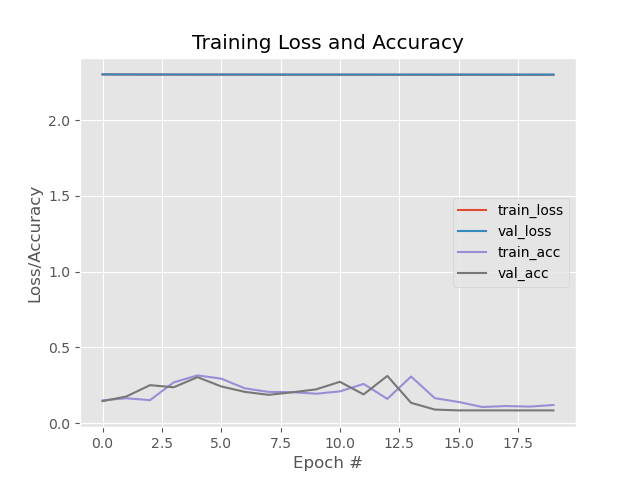
\includegraphics[width=0.8\textwidth]{epochs20_div255}
  \caption{Divide 255 and epochs=20}
  \label{fig:div255-epochs20}
\end{figure}


\begin{figure}[!ht]
  \centering
  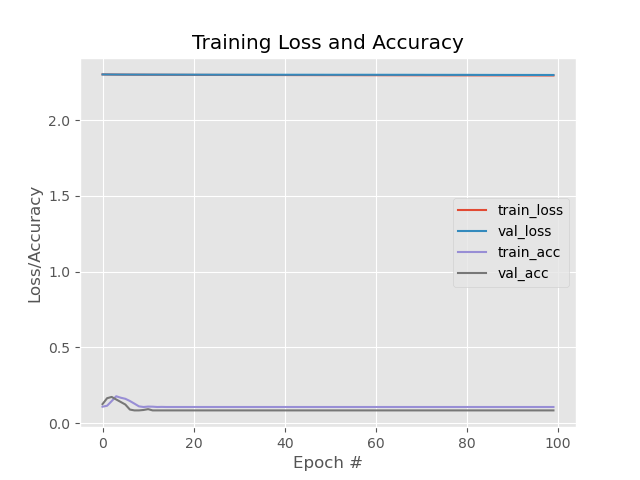
\includegraphics[width=0.8\textwidth]{epochs100_div255}
  \caption{Divide 255 and epochs=100}
  \label{fig:div255-epochs100}
\end{figure}


After diving into the dataset, I found that the maximum value is 16.
After changing the division to 16, the result is shown in Figure \ref{fig:div16-epochs20}.

\begin{figure}[!ht]
  \centering
  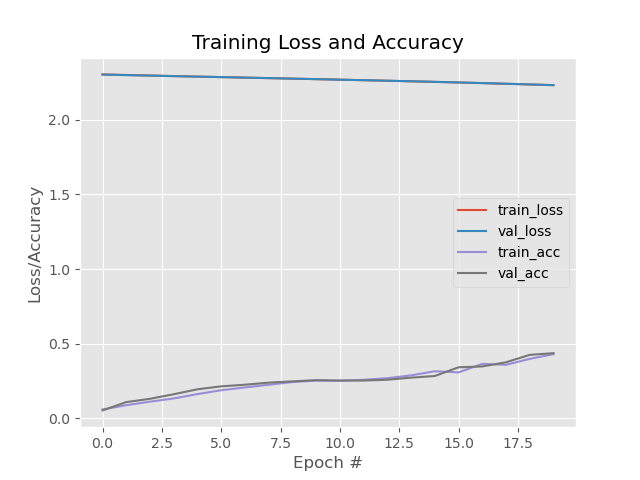
\includegraphics[width=0.8\textwidth]{epochs20_div16}
  \caption{Divide 16 and epochs=20}
  \label{fig:div16-epochs20}
\end{figure}


From the Figue \ref{fig:div16-epochs20} we can see that the epochs is too small.
After chaning the epochs to 100, the result is shown inf Figure \ref{fig:div16-epochs100}.
\begin{figure}[!ht]
  \centering
  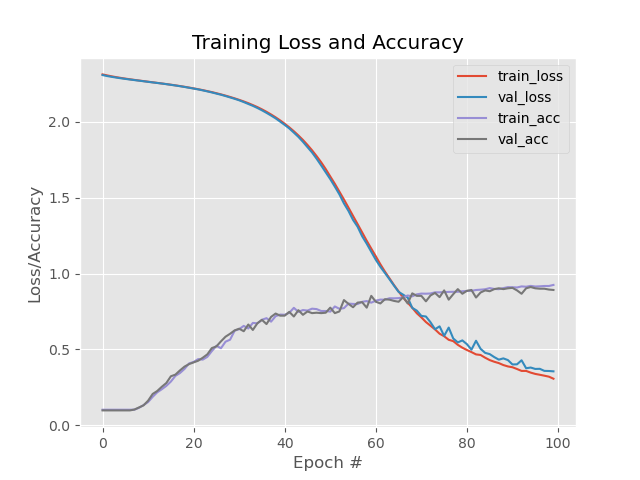
\includegraphics[width=0.8\textwidth]{epochs100_div16}
  \caption{Divide 16 and epochs=100}
  \label{fig:div16-epochs100}
\end{figure}


\section{LeNet with PyTorch}
\label{sec:lenet-with-pytorch}

The code link on \href{https://github.com/mingmingli916/dl_classification}{Github}.

Before, there is no tensorboard in PyTorch. You did the training process visualization.
With the tensorboard, it becomes more easier for the visualization in training process.



%%% Local Variables:
%%% mode: latex
%%% TeX-master: "deep-learning"
%%% End:
